\section*{Supplementary material}
\setcounter{table}{0}\setcounter{figure}{0}
\renewcommand{\thetable}{S\arabic{table}}
\renewcommand{\thefigure}{S\arabic{figure}}

\begin{table}[h]
\centering
\caption{Representation used for each pair.}
\label{tab:reps}
\todo{Table S1: PCA / scGPT-spatial per pair (methods.md \S4)}
\end{table}

\begin{table}[h]
\centering
\caption{Per-class reference floor, USHER-ST configuration, four COAD pairs $\times$ three seeds, held-out tiles.
The floor was selected on a validation split of the training tiles by a rule fixed in advance: the largest rare-type
purity among floors losing no more than 0.02 in xfer\_main or total score. That rule chose 200.}
\label{tab:floor}
\small
\begin{tabular}{@{}lcccccc@{}}
\toprule
Floor & xfer\_main & xfer\_all & rare\_purity & batch\_v2 & bio\_v2 & total\_v2 \\
\midrule
0    & 0.7210 & 0.4284 & 0.2201 & 0.6052 & 0.7020 & 0.6633 \\
200  & 0.7229 & 0.4420 & 0.2405 & 0.6114 & 0.7049 & 0.6675 \\
500  & 0.7291 & 0.4485 & 0.2547 & 0.6106 & 0.7048 & 0.6671 \\
1000 & 0.7289 & 0.4551 & 0.2626 & 0.6109 & 0.7058 & 0.6678 \\
\bottomrule
\end{tabular}
\end{table}

\begin{figure}[h]
\centering
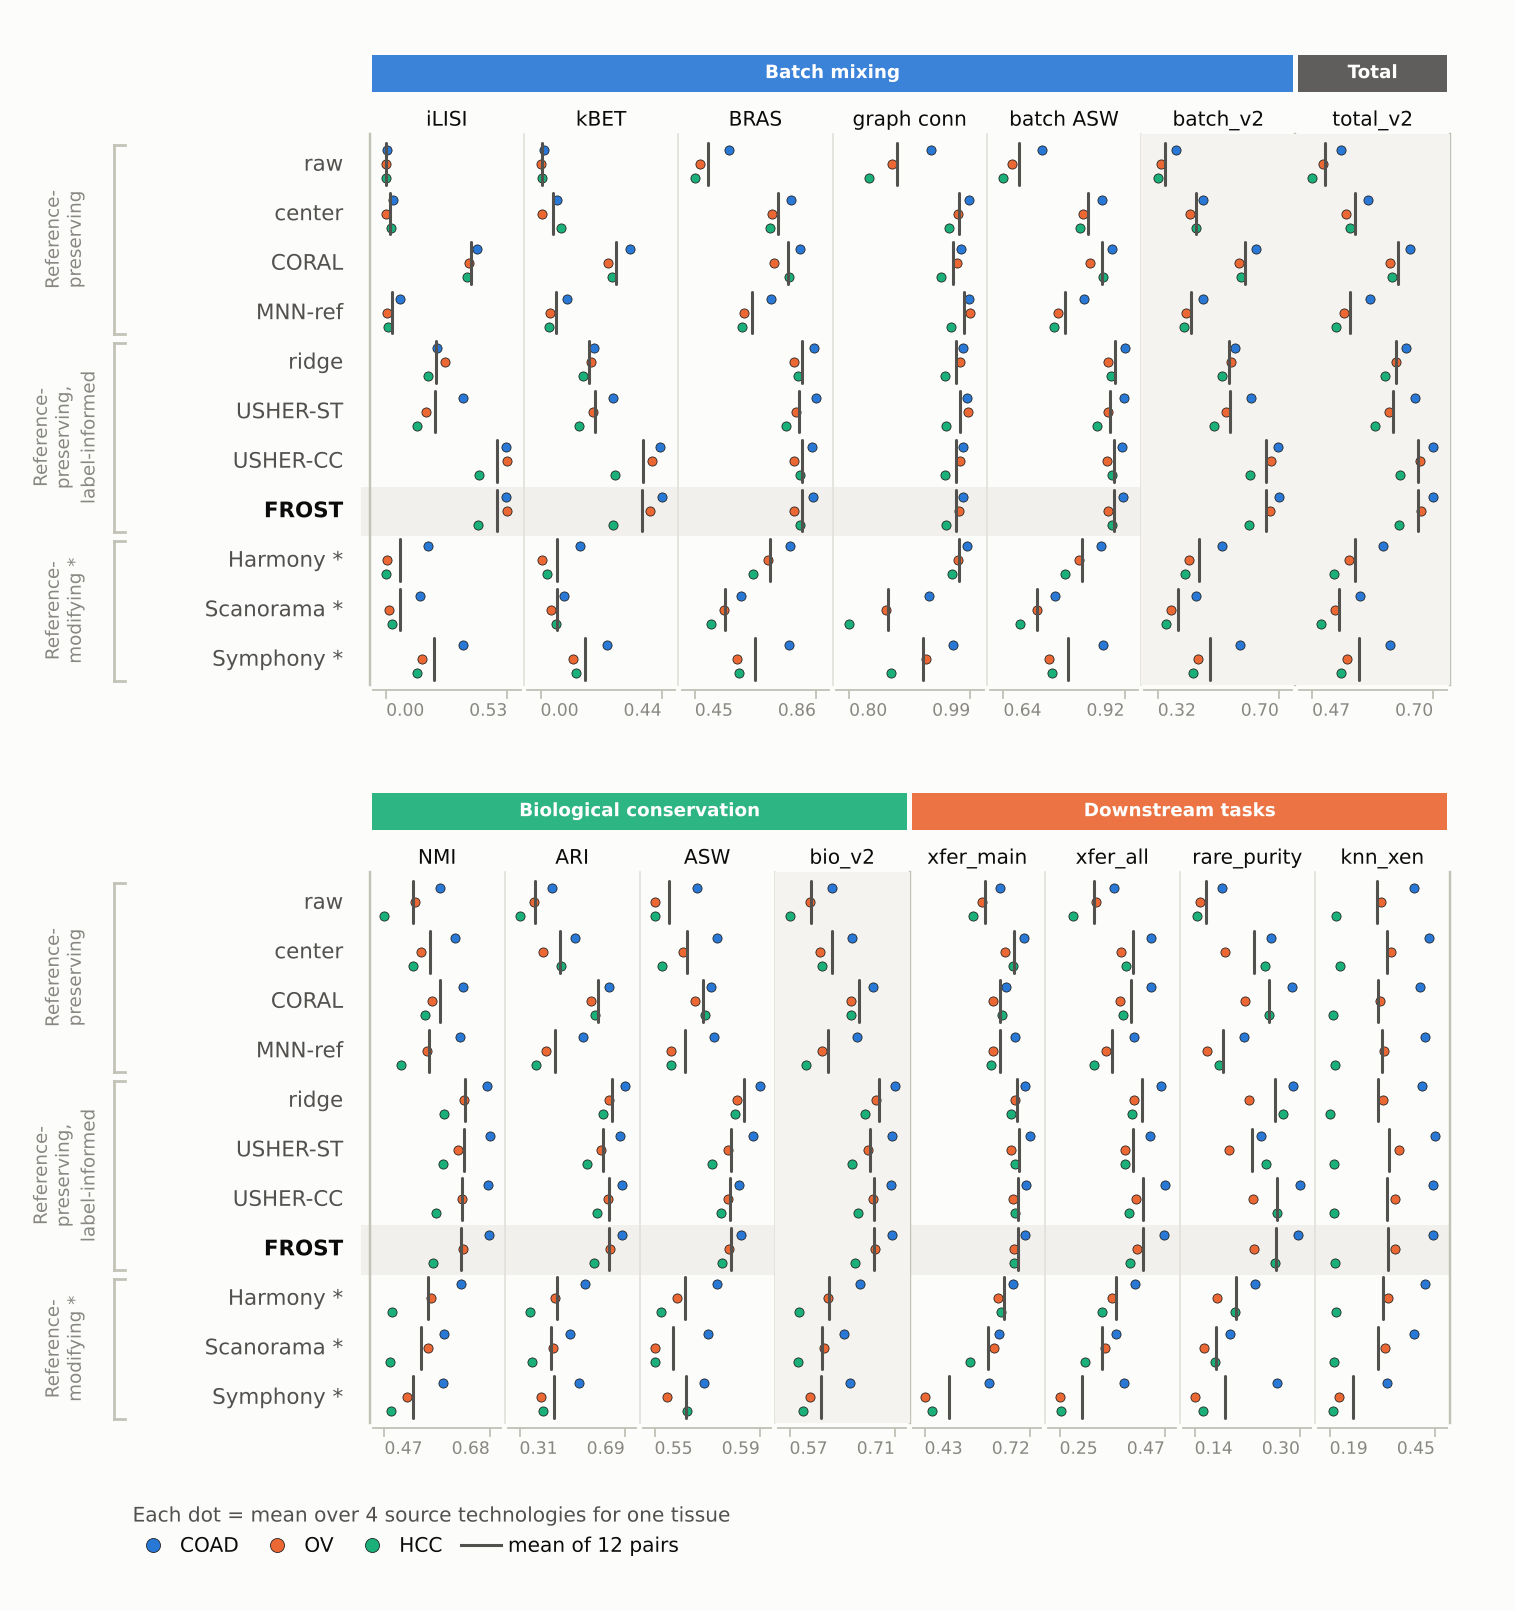
\includegraphics[width=\linewidth]{figs/fig_grid_tissue.png}
\caption{As Figure~\ref{fig:grid}, but each dot is the mean over four source technologies for one tissue.}
\label{fig:grid_tissue}
\end{figure}
